\documentclass{article}

% if you need to pass options to natbib, use, e.g.:
%     \PassOptionsToPackage{numbers, compress}{natbib}
% before loading neurips_2020

% ready for submission
% \usepackage{neurips_2020}

% to compile a preprint version, e.g., for submission to arXiv, add add the
% [preprint] option:
\usepackage[preprint]{neurips_2020}

% to compile a camera-ready version, add the [final] option, e.g.:
%   \usepackage[final]{neurips_2020}

% to avoid loading the natbib package, add option nonatbib:
%    \usepackage[nonatbib]{neurips_2020}

\usepackage[utf8]{inputenc} % allow utf-8 input
\usepackage[T1]{fontenc}    % use 8-bit T1 fonts
\usepackage{hyperref}       % hyperlinks
\usepackage{url}            % simple URL typesetting
\usepackage{booktabs}       % professional-quality tables
\usepackage{amsfonts}       % blackboard math symbols
\usepackage{nicefrac}       % compact symbols for 1/2, etc.
\usepackage{microtype}      % microtypography
\usepackage{lineno}
\usepackage{graphicx}
\usepackage{subfigure}
\usepackage{caption}
\usepackage{cleveref}
\linenumbers


\title{Evaluate and Switch between LaTeX and Natural Mathematical Expressions with Encoder-Decoder}
% EASyNet: Equivalence Accessment System
\author{
    Zeyun Wu\\
    Department of Electrical and Computer Engineering \\
    University of California, San Diego \\
    La Jolla, CA 92093 \\
    \texttt{zew038@ucsd.edu}
}


\begin{document}
    
\maketitle

\begin{abstract}
This paper introduces a pilot study of evaluating and translation between LaTeX and natural mathematical expressions. We implemented algorithms that generate LaTeX and natural expressions by defining rules and permutating elements. We utilized encoder-decoder networks with attention mechanism to translate LaTeX expression to natural expression with high performance. Some critiques and future direction were discussed and the study was still preliminary. 
\end{abstract}

\section{Introduction}
LaTeX (\LaTeX) is a typesetting software system that allows users to gain scalable, systematic, and consistent presentation of contents. It is commonly used by people from all fields in various circumstances, including writing this paper. It is especially useful in formatting mathematical expressions. For instance, this is an example of well-organized presentation of LaTeX equation computing gradient during backpropagation when training neural network. \par 
\[ \nabla_{\mathbf{w}^l} L[\eta(x; \theta), y] = \frac{\partial L[\eta(x; \theta), y]}{\partial z^l} \frac{\partial z^l}{\partial \mathbf{w}^l} \]
While LaTeX is a great application for composings written documentation, during daily communication, we constantly use natural language expressions to describe our thoughts. It would be naturally interesting and useful to explore the following two major tasks: translation between LaTeX and natural expression, and evaluate whether a given pair of LaTeX and natural expressions is equivalent to each other. To fulfill these two tasks, we utilized encoder-decoder networks with attention, which is one of state-of-the-art algorithms in natural language translation. \par 
Currently, there had been a lot of study about converting images of mathematical expression into LaTeX. However, there is no study about convertion between LaTeX and natural expressions yet. Moreover, there is no available public dataset for similar tasks. Therefore, we also developed methods to generate LaTeX and natural expression pairs. 
% 
%
\section{Dataset}
\begin{table}
    \caption{Elements used in generating expression pairs}
    \label{element}
    \centering
    \begin{tabular}{|p{3cm}||p{8cm}|  }
        \hline
        Types& Elements in Corresponding Type \\
        \hline
        \hline
        Digit (for LaTeX)& 0, 1, 2, 3, 4, 5, 6, 7, 8, 9   \\
        \hline
        Number (for natural)& zero, one, two, three, four, five, six, seven, eight, nine \\
        \hline
        Variable & x, y, z \\
        \hline
    \end{tabular}
\end{table}
%
Currently, there is no public data that can be used in the tasks we would like to explore. Thus, we implemented methods to generate pairs of equivalent LaTeX and natural expressions (in English) from pre-defined rules and elements. \par 
By default, we treated all LaTeX expressions as under math mode. We first defined limited number of possible operations including plus, minus, power, fraction, integral, etc, as well as elements (Table~\ref{element}). We then defined three types of rules to write expression pairs. By permutating elements in defined rules, we generated over 3000 pairs of equivalent expressions.
%
\subsection{Define Expression Rules}
\begin{table}
  \caption{Examples of rules for generating base and complex expression pairs. Numbers are placeholder representing elements to be filled. There can be several different natural expressions for the same LaTeX expression, which are separated by `;'.}
  \label{rule}
  \centering
  \begin{tabular}{|p{1.5cm}||p{3.5cm}|p{7cm}|}
      \hline
      Types& LaTeX rule & Natural rule \\
      \hline
      \hline
      Base & 0 \textbackslash ge 1 & 0 is greater or equal to 1 \\
      \hline 
      Base& \textbackslash frac\{0\}\{1\} & 0 over 1; 0 divided by 1 \\
      \hline
      Base& 0\textbackslash times 1 & 0 times 1; 1 multiplied by 0; product of 0 and 1 \\
      \hline
      Complex& \textbackslash int\_\{0\}\^ \ \{1\} h(2) \textbackslash,d3 & integral of h ( 2 ) from 0 to 1 with respect to 3 \\
      \hline
      Complex& \textbackslash lim\_\{0 \textbackslash to 1\} h(2) & limit of h ( 2 ) as 0 goes to 1 \\
      \hline
  \end{tabular}
\end{table}
%
There are three types of rules: base, complex, and nested. Some of the examples were listed in Table~\ref{rule}. \par 
Base rules were the most basic and simple rules. They consisted of basic operations: plus, minus, multiplicatiom, fraction, power, and comparations. They had two or less parameters, and tended to have the most simple grammar in both LaTeX and natural expressions. Note there can be several different but equivalent natural expressions for one single LaTeX expression. For example, for multiplication, people would say one times two, or two multiplied by one, or product of one and two. \par 
Complex rules generally were relatively complicated. They often had three or more parameters, and were with complex grammer. There were less number of complex rules than base rules. \par 
Nested expressions were composed by nesting multiple base expressions or complex expressions. For base and complex rule, they were filled by elements, while nested expressions were filled by base or complex expressions. For example, we can have `\textbackslash frac\{x+1\}\{x\} \textbackslash ne 1' and `x plus one over x is not equal to one' as a nested pair. Nested data was not used during training. Rather, they were used only during testing stage. 
%
\subsection{Data Generation}
With defined rules, we generated expression pairs by permutating appropriate elements in corresponding placeholder positions. Generally all possible cartesian products of elements would be used to generate expression pairs. However, for positions of some rules, only one type of elemenets were legit. For example, in interal expression, the boundaries can only be filled with elements in Digit type (in LaTeX) or Number type (in natural), and the vairable can only be filled with elements in Variable type (see Table~\ref{element} and ~\ref{rule}). \par 
In total, we generated 3391 data pairs which would be used during training, along with several nested pairs. We shuffle all the expression pairs and split 80\% of the pairs into training set, and rest into testing set. Again, nested expressions were not used during training. 
%
\section{Experiment}
%
\subsection{Tokenization}
Before we can feed data into networks, we would need to define token for both LaTeX and natural languages. 
%
\subsection{Encoder-Decoder with Attention}
%
%
\section{Result}
\begin{figure}[h]
  \centering
  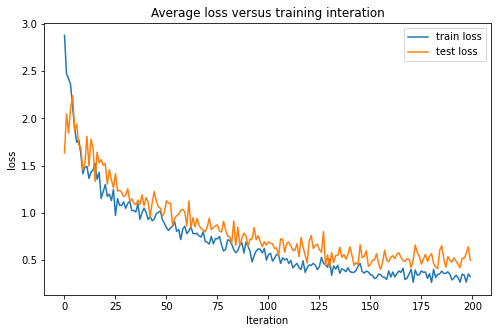
\includegraphics[width=12cm]{../plot/loss_curve.png}
  \caption{Training and testing loss curves versus training iteration}
  \label{fig:loss}
\end{figure}
%
\section{Discussion}


    
%%%%%%%%%%%

\section*{References}

\small

[1] https://www.kaggle.com/austinreese/craigslist-carstrucks-data



\end{document}
